\section{Genetsko programiranje}
\emph{Genetsko programiranje} (\emph{GP}) je evolucijski algoritam koji do rješenja dolazi iterativno mjenjajući populaciju sve dok uvjet zaustavljanja nije zadovoljen (\cite{conv_gen_programming}).

Inspiraciju vuče iz prirode.
Algoritam počinje s nasumično nastalom populacijom koja se poboljšava kroz ograničen broj generacija.
Nastanak svake generacije započinje izborom jedinki (detaljno opisane u nastavku).
Izbor nije nasumičan niti determinističan, boljim jedinkama daje se prednost pri izboru no i one lošije mogu biti izabrane.
Nedeterminističnost izbora rezultira širem pretraživanju prostora rješenja, ne ograničenim samo na najbolje jedinke.
Iz jedinki nastaju nove kao rezultat genetskih operatora \emph{Križanja} i \emph{Mutacije}.
Ciklus se ponavlja sve dok jedna od dvije stvari nije zadovoljena:
\begin{itemize}
	\item{Dosegnut najveći broj iteracija ili evaluacija}
	\item{Postignuta željena preciznost rješenja (npr. $greska \leq 10^{-3}$})
\end{itemize}
Na kraju postupka, dobiveni model osim što se može koristiti u željenu svrhu, lako se može izučiti i interpretirati, jer za razliku od neuronskih mreža, način na koji ulaz postaje izlaz jasno je čitljiv. \\
Jednostavan primjer genetskog algoritma vidljiv je u pseudokodu ~\ref{alg:gp_example}

\begin{algorithm}
	\caption{Jednostavni genetski algoritam (\cite{wong2015evolutionary})}
	\label{alg:gp_example}
	\begin{algorithmic}
		\STATE $P(t)$: Roditeljska populacija u generaciji $t$
		\STATE $O(t)$: Populacija potomaka u generaciji $t$
		\STATE $P(t)=$ stvori\_pocetnu\_populaciju()
		\WHILE{uvjet zaustavljanja nije zadovoljen}
			\STATE $P^{'}(t) =$ izabrani roditelji iz $P(t)$
			\STATE $O(t + 1) =$ potomci nastali krizanjem jedinki iz $P^{'}(t)$
			\STATE $O(t + 1) = mutiraj\ O(t + 1)$
			\STATE $evaluiraj(O(t + 1))$
			\STATE $P(t + 1) = O(t + 1)$
			\STATE $t = t + 1$
		\ENDWHILE
	\end{algorithmic}
\end{algorithm}

\subsection{Jedinka populacije}
Jedinka populacije u genetskom algoritmu predstavlja jedno moguće rješenje na problem koji smo postavili.
Svaka jedinka je definirana s dvije stavke:
\begin{itemize}
	\item{Genotipom}
	\item{Načinom mapiranja genotipa u \emph{fenotip}}
\end{itemize}
Na najnižoj razini, svaka jedinka je jedan genotip. 
U praksi, genotip može biti prikazan na bilo koji način koji odgovara korisniku algoritma, no neke od najčešćih struktura su vektori brojeva, simbola ili bitova, fiksne ili varijabilne duljine, te stablaste strukture (\cite{naturally_selecting_algorithms}).
Korisnik koji koristi \emph{genetski algoritam} (GA) za pronalazak rješenja mora također definirati mapiranje $genotip \rightarrow fenotip$.
Genotipom možemo smatrati ono što koristi algoritam kako bi stvorio fenotip, dok je fenotip jedno od mogućih rješenja na problem koji rješavamo.
Što to znači?
Ukoliko je zadatak GA iz skupa točaka provesti simboličku regresiju $A\sin(Bx + C)$ gdje su $A$, $B$ i $C$ nepoznate varijable genotip bi se mogao prikazati kao vektor s broja s pomičnim zarezom.
Dalje, pravilo mapiranja genotipa u fenotip bi moglo biti da element na prvom mjestu odgovara vrijednosti koju pridajemo varijabli $A$ i tako dalje za varijable $B$ i $C$ (~\ref{fig:genotype_phenotype_map}).
Također, bitno je kvantificirati kvalitetu jedinke.
Ta mjera najčešće se naziva kondicija (\emph{eng. fitness}).
Sve jedinke populacije dobivaju kondiciju na temelju istog pravila kako bi bili međusobno usporedivi.
Jedinka s najvećom kondicijom smatra se najkvalitetnijom i najboljim rješenjem na problem koji se rješava.

\begin{figure}
	\caption{Mogućnosti spremanja i korištenja genotipa tijekom izvođenja genetskog algoritma}
	\begin{subfigure}[t]{0.45\textwidth}
		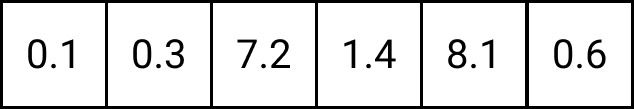
\includegraphics[width=\textwidth]{Illustrations/float_genotype.png}
		\caption{Genotip prikazan brojem s pomičnim zarezom}
	\end{subfigure}
	\hspace{\fill}
	\begin{subfigure}[t]{0.45\textwidth}
		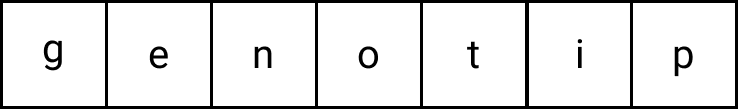
\includegraphics[width=\textwidth]{Illustrations/char_genotype.png}
		\caption{Genotip prikazan ascii znakovima}
	\end{subfigure}
	\label{fig:genotype_types}
\end{figure}

\begin{figure}
	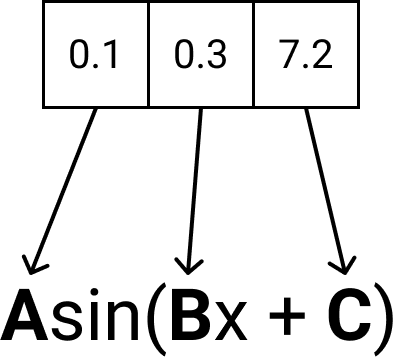
\includegraphics[width=0.4\linewidth]{Illustrations/genotype_phenotype_mapping.png}
	\caption{Primjer mapiranja genotipa u fenotip}
	\label{fig:genotype_phenotype_map}
\end{figure}

\subsection{Genetski operatori}
Genetski operatori pružaju osnovni mehanizam pretrage genetskog algoritma.
Za zadatak imaju stvarati nova rješenja uz efektivnu pretragu prostora rješenja.
Izvode se na primitivu jedinki, genotipu, te se nerjetko međusobno izvode u kombinaciji jer samostalno nisu uvijek efektivni.
U nastavku su opisane 2 osnovne vrste genetskih operatora, križanje i mutacija.

\subsubsection{Križanje}
Operator križanja u genetskom algoritmu oponaša reprodukciju u biološkom svijetu.
Od dvije jedinke stvara nove primjenjujući neko definirano pravilo kombinacije njihovih genotipa.
Križanje nije trivijalno kao na prvi pogled, te je usko ovisno o izboru strukture podataka s kojom definiramo genotip (~\cite{wong2015evolutionary}). \\
Na slici ~\ref{fig:crossover} prikazan je primjer jednog od operatora križanja koje ću detaljnije opisati u nastavku.

\begin{figure}
	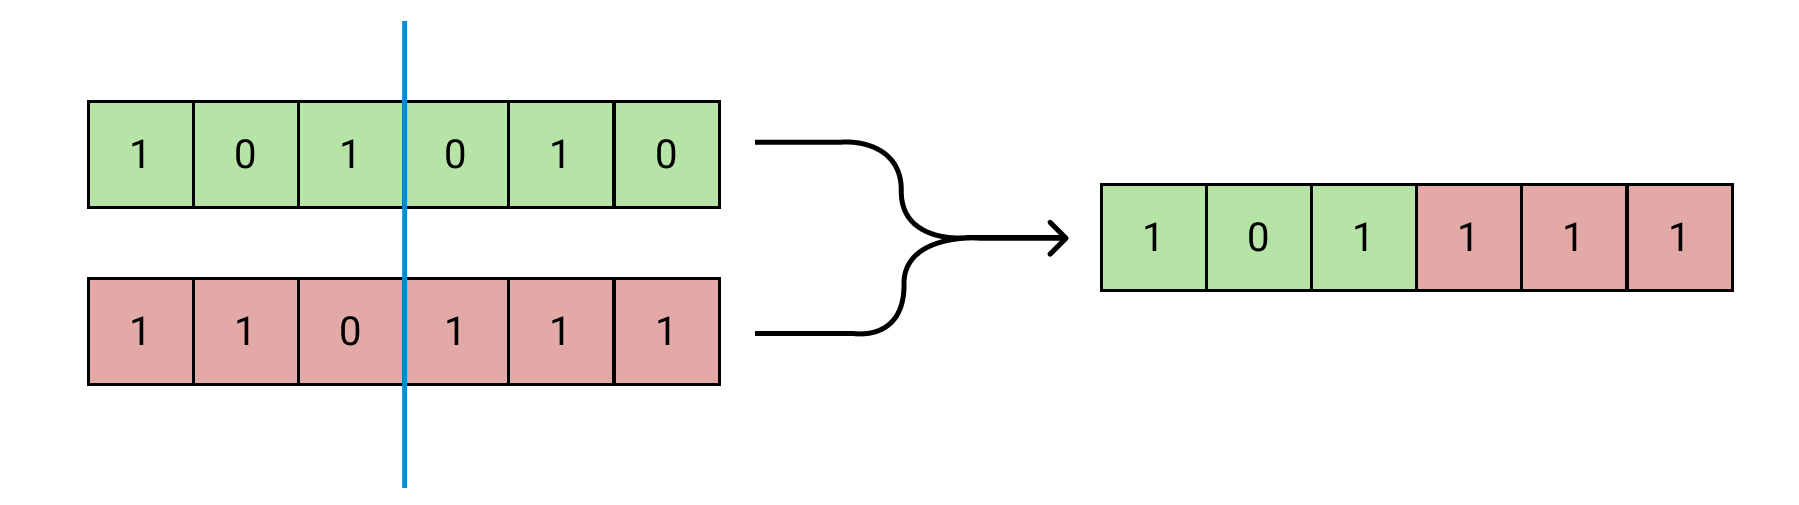
\includegraphics[width=\linewidth]{Illustrations/crossover.png}
	\caption{Jednostavni primjer rezultata primjene operatora križanja}
	\label{fig:crossover}
\end{figure}

\paragraph{Križanje u k točaka}
se koristi tako da se odabere $k$ nasumičnih točaka koje služe kao granica između kojih se uzimaju dijelovi dva različita genotipa.
Često se odabere $k = 1$ (primjer na slici ~\ref{fig:crossover}) zbog svoje jednostavnosti.
Ono što se često zamjera križanju u jednoj točki je pristranost poziciji genotipa.
To znači da će pri odabiru dva roditeljska genotipa $P_1$ i $P_2$ lijevi dio novonastalog genotipa uvijek pripasti pripadajućem dijelu $P_1$ a desni $P_2$.
Rješenje na taj problem, osim odabira $k > 1$, je stvaranje dva potomka koja se zatim evaluiraju, nakon čega se potomak koji se pokaže boljim prenosi u sljedeću generaciju populacije (ilustracija ~\ref{fig:position_bias}).

\begin{figure}
	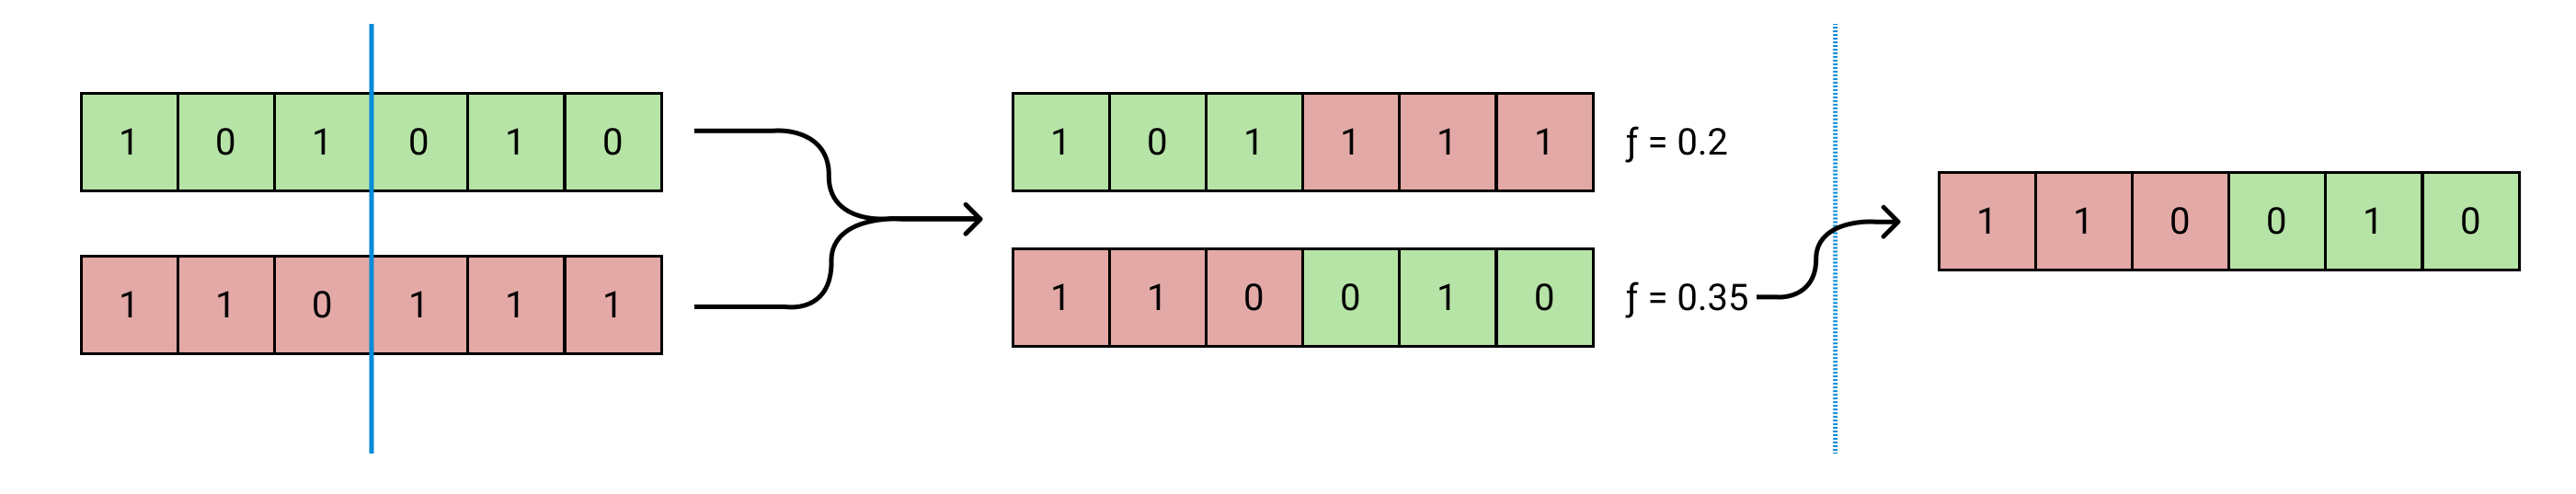
\includegraphics[width=\linewidth]{Illustrations/position_bias.png}
	\caption{Primjer rješavanja problema pristranosti pozicije}
	\label{fig:position_bias}
\end{figure}

\paragraph{Ujednačeno križanje}
tretira svaki gen u genotipu zasebno što osigurava da svaki roditeljski gen ima jednaku šansu da se prenese na novonastali genotip.
Postupak se može definirati kao:
\[
	O[n] = \left\{\begin{array}{lr}
			P_1[n], & \text{za } 0 \leq \alpha \leq 0.5 \\
			P_2[n] & \text{za } 0.5 < \alpha \leq 1
		\end{array}\right\}
\]
Također, grafički prikazano na ilustraciji ~\ref{fig:uniform_crossover}.

\begin{figure}
	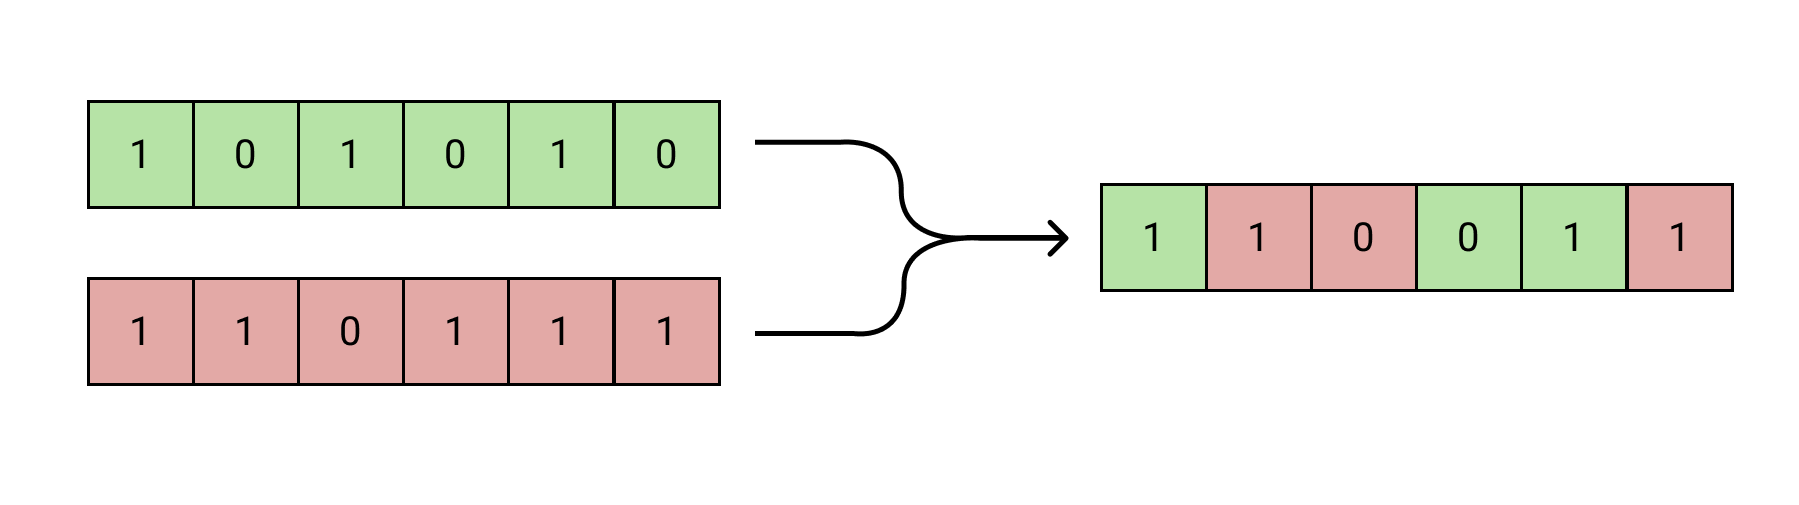
\includegraphics[width=\linewidth]{Illustrations/uniform_crossover.png}
	\caption{}
	\label{fig:uniform_crossover}
\end{figure}
